\documentclass[12pt]{article}
\usepackage{light}

\hidesolutions
%\showsolutions

\begin{document}

\recitation{20}{November 16, 2012}

%%%%%%%%%%%%%%%%%%%%%%%%%%%%%%%%%%%%%%%%%%%%%%%%%%%%%%%%%%%%%%%%%%%%%%%%%%%%%%%

\section*{The Four-Step Method}

This is a good approach to questions of the form, ``What is the
probability that ------?''  Intuition \textit{will} mislead you, but
this formal approach gives the right answer every time.

\begin{enumerate}
\item Find the sample space.  (Use a tree diagram.)

\item Define events of interest.  (Mark leaves corresponding to these
events.)

\item Determine outcome probabilities:

\begin{enumerate}

\item Assign edge probabilities.

\item Compute outcome probabilities.  (Multiply along root-to-leaf
paths.)

\end{enumerate}

\item Compute event probabilities.  (Sum the probabilities of all
outcomes in the event.)

\end{enumerate}

%%%%%%%%%%%%%%%%%%%%%%%%%%%%%%%%%%%%%%%%%%%%%%%%%%%%%%%%%%%%%%%%%%%%%%%%%%%%%%%

\newpage


\section{The Four-Door Deal}

Suppose that {\em Let's Make a Deal} is played according to different
rules.  Now there are \underline{four} doors, with a prize hidden
behind one of them.  The contestant is allowed to pick a door.  The
host must then reveal a different door that has no prize behind it.
The contestant is allowed to stay with his or her original door or to
pick one of the other two that are still closed.  If the contestant
chooses the door concealing the prize in this second stage, then he or
she wins.

\begin{enumerate}
\item Contestant Stu, a sanitation engineer from Trenton, New Jersey,
stays with his original door.  What is the probability that he wins
the prize?

The tree diagram is awkwardly large.  This often happens; in fact,
sometimes you'll encounter \textit{infinite} tree diagrams!  Try to
draw enough of the diagram so that you understand the structure of the
remainder.

\solution[\newpage]{Let's make the following assumptions:
%
\begin{enumerate}
\item The prize is equally likely to be behind each door.
\item The contestant is equally likely to pick each door initially,
regardless of the prize's location.
\item The host is equally likely to reveal each door that does not
conceal the prize and was not selected by the player.
\end{enumerate}
%
A partial tree diagram is shown below.  The remaining subtrees are
symmetric to the full-expanded subtree.
%
\begin{center}
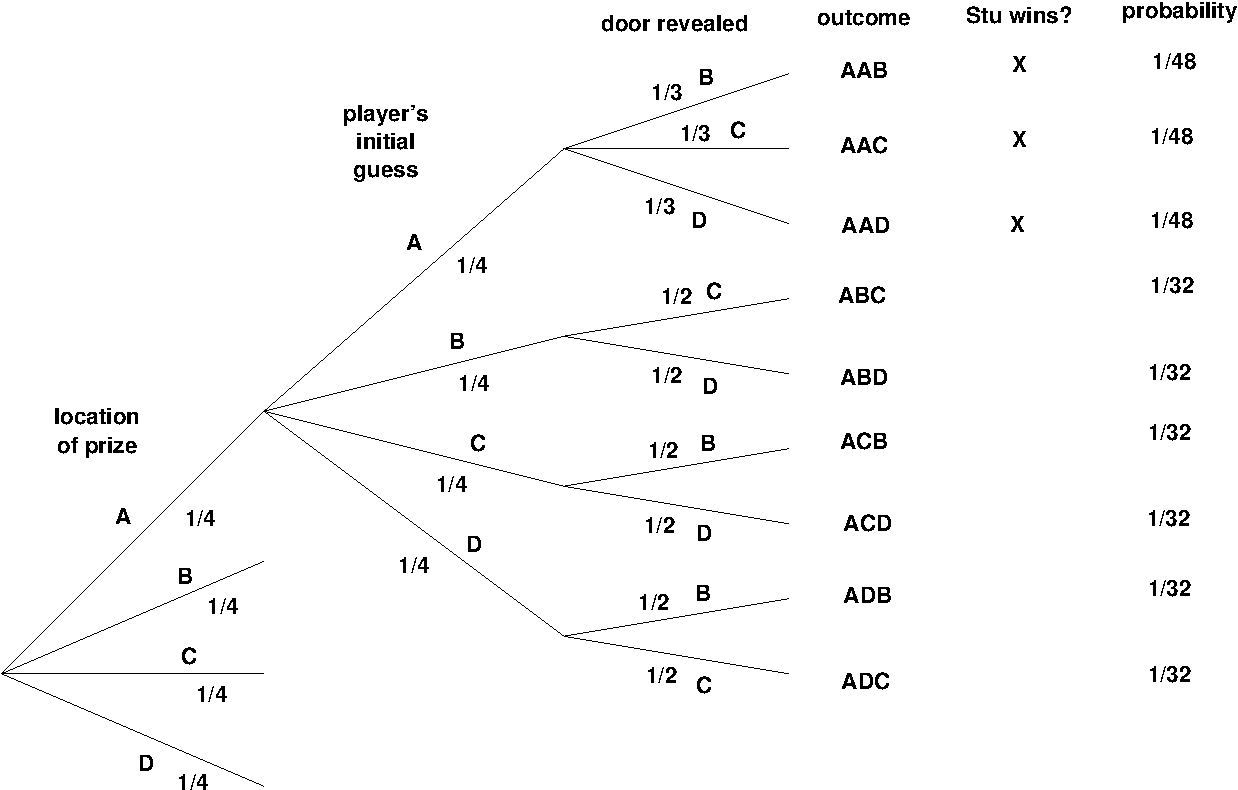
\includegraphics[width=6in]{four-door}
\end{center}
%
The probability that Stu wins the prize is:
%
\[
\pr{\text{Stu wins}} = 4 \cdot \left(\frac{1}{48} + \frac{1}{48} + \frac{1}{48}\right) = \frac{1}{4}
\]
%
We multiply by 4 to account for the four subtrees, of which we've only
drawn one.}

\item Contestant Zelda, an alien abduction researcher from Helena,
Montana, switches to one of the remaining two doors with equal
probability.  What is the probability that she wins the prize?

\solution{A partial tree diagram is worked out below.
%
\begin{center}
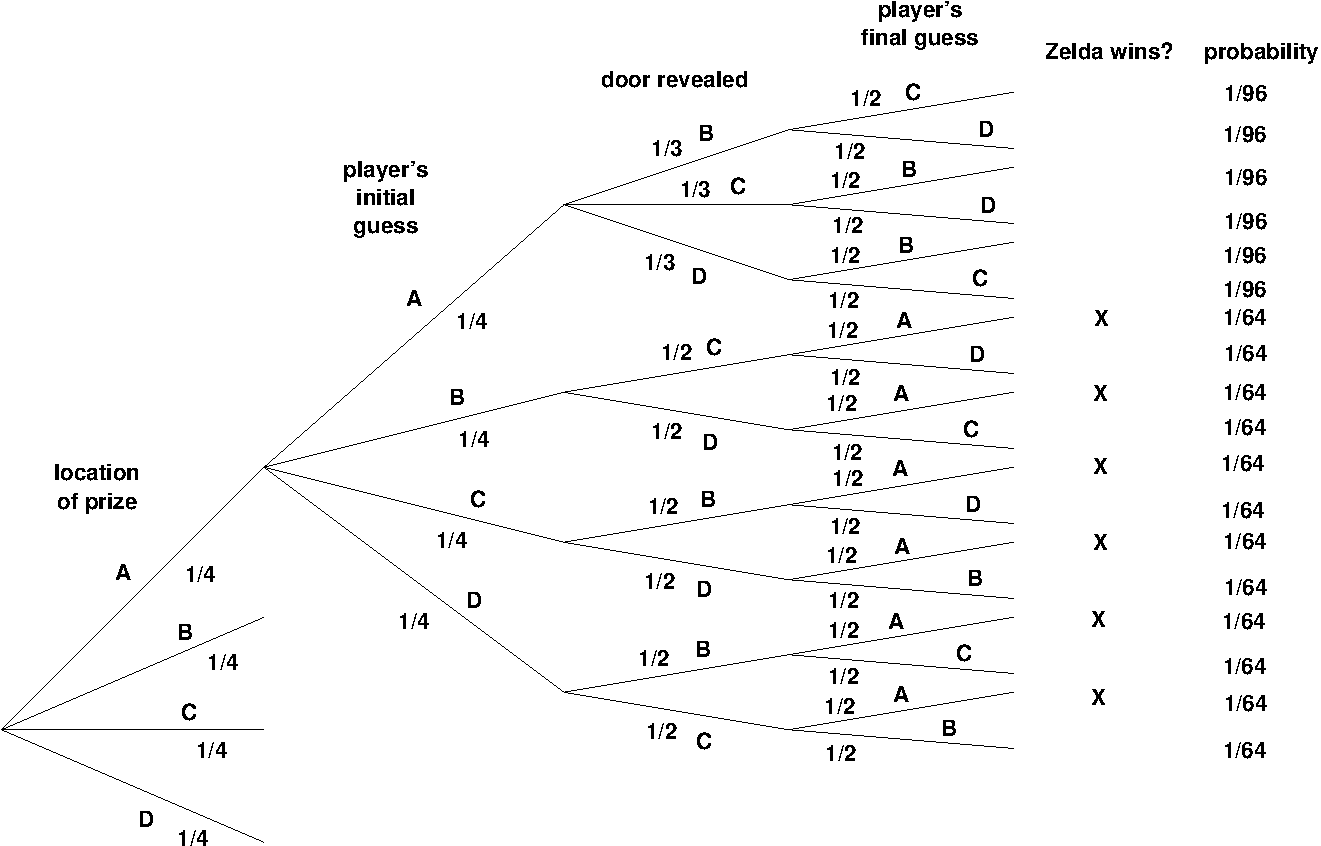
\includegraphics[width=6in]{four-doorb}
\end{center}
%
The probability that Zelda wins the prize is:
%
\[
\pr{\text{Zelda wins}} = 4 \cdot \left( \frac{1}{64} + \frac{1}{64} + \frac{1}{64} + \frac{1}{64} + \frac{1}{64} + \frac{1}{64} \right) = \frac{3}{8}
\]
}
\end{enumerate}

%%%%%%%%%%%%%%%%%%%%%%%%%%%%%%%%%%%%%%%%%%%%%%%%%%%%%%%%%%%%%%%%%%%%%%%%%%%%%%%

\newpage

\section{Earliest Door}

Let's consider another variation of the four-doors problem.  Say the
doors are labeled A, B, C, and D.  Suppose that Carol always opens the
\textit{earliest} door possible (the door whose label is earliest in
the alphabet) with the restriction that she can neither reveal the
prize nor open the door that the player picked.

This gives contestant Mergatroid--- an engineering student from
Cambridge, MA--- just a little more information about the location of
the prize.  Suppose that Mergatroid always switches to the earliest
door, excluding his initial pick and the one Carol opened.  What is
the probability that he wins the prize?

%% (Interestingly, in the three-door problem, the contestant gains no
%% advantage if Carol always opens the earliest door available.  In
%% other words, if the contestant uses the best possible strategy, his
%% changes of winning are still two in three.)

\solution{
A tree diagram is worked out below.
%
\begin{center}
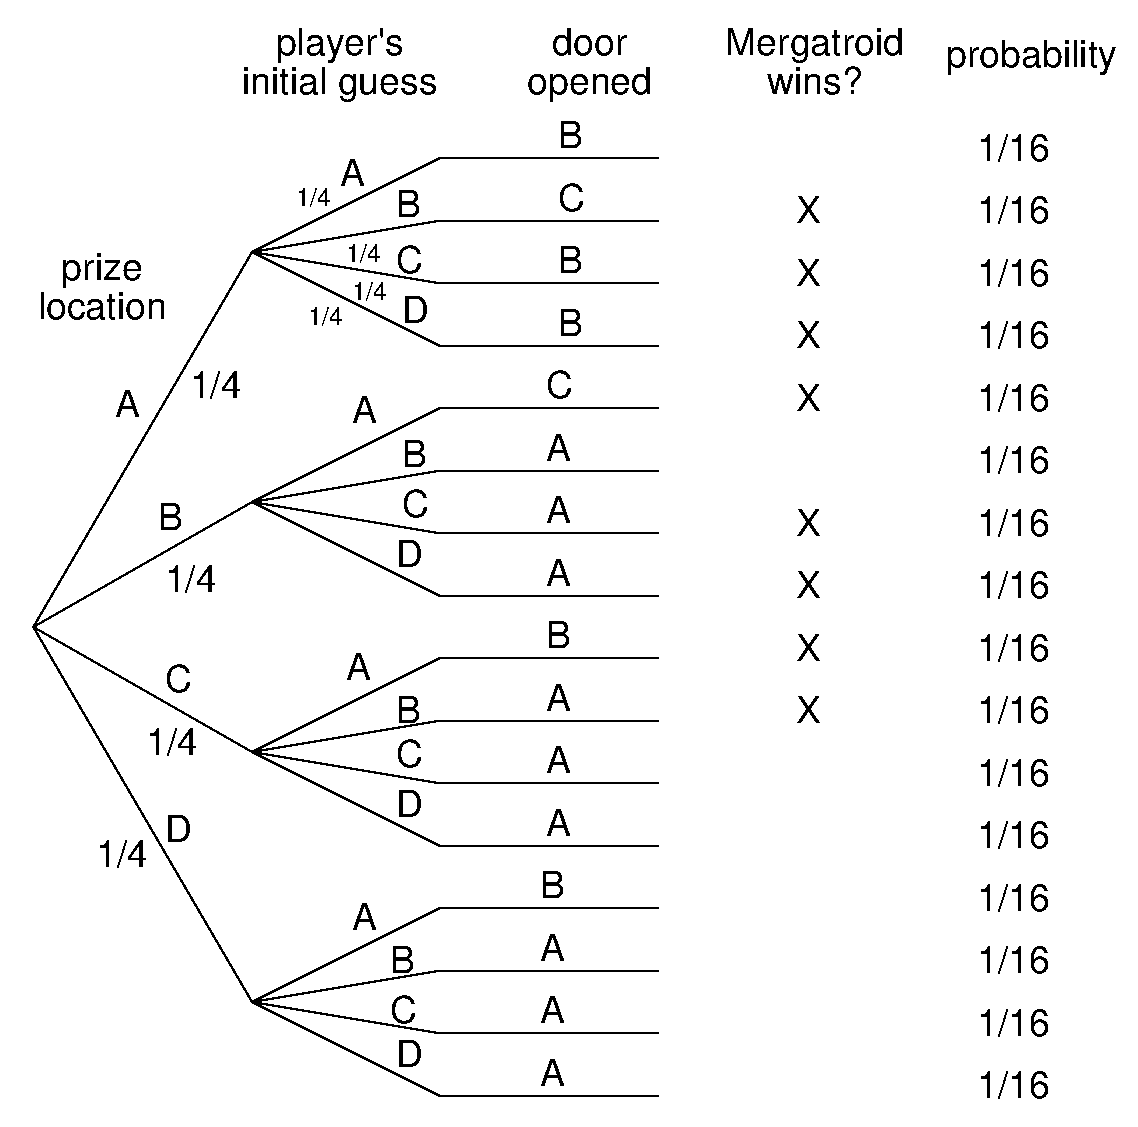
\includegraphics[height=3.5in]{carol}
\end{center}
%
The probability that Mergatroid wins is:
%
\[
\pr{\text{win}} = 8 \cdot \frac{1}{16} = \frac{1}{2}
\]
}

%%%%%%%%%%%%%%%%%%%%%%%%%%%%%%%%%%%%%%%%%%%%%%%%%%%%%%%%%%%%%%%%%%%%%%%%%%%%%%%
\newpage
\section{The 3 doors version revisited}

\subsection{Carol picks the smallest door} 

Suppose we are in the original game show with 3 doors. In our original analysis we assumed Carol picked the door randomly. In this case suppose Carol picks the smallest door, while still making sure of both i) it contains a goat and ii) it is not the contestants first choice. The contestant follows the switching strategy. What is the probability the contestant wins? 

\solution{
A tree diagram is worked out below.

\begin{center}
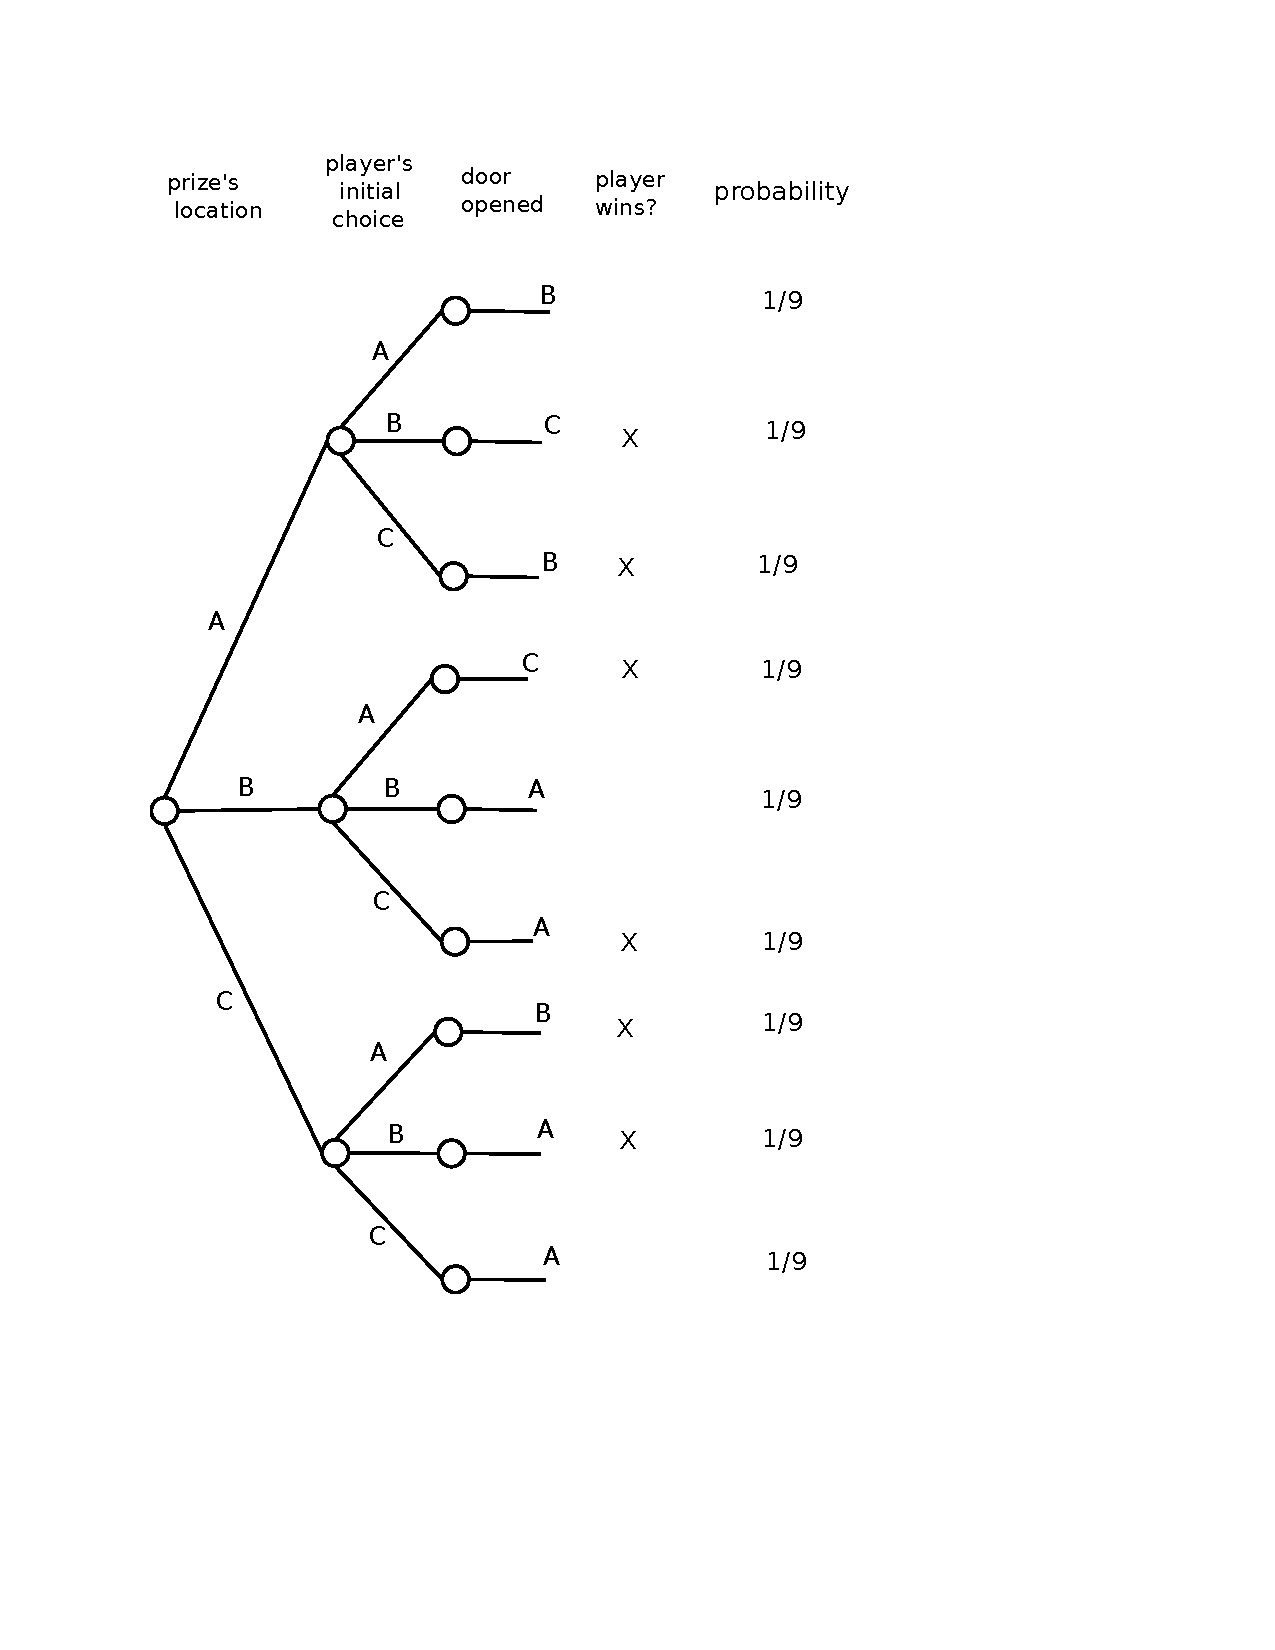
\includegraphics[scale=0.7]{threeleft}
\end{center}

Hence the probability of winning using the switch strategy is $2/3$, even when Carol picks the earliest door possible.  This is also the case using Mergatroid's strategy of switching to the leftmost option. There is always only one option left over, so only one option to switch to anyway. Contrast this to the 4 door case worked out before.

}

\subsection{Carol picks the smallest door with probability $p$} 
This time, when Carol has a choice she chooses the smallest possible door with probability $p$ and the other remaining door with probability $1-p$.  The contestant still follows the switching strategy. What is the probability the contestant wins, in terms of $p$?

\solution{
Observe the tree diagram below:

\begin{center}
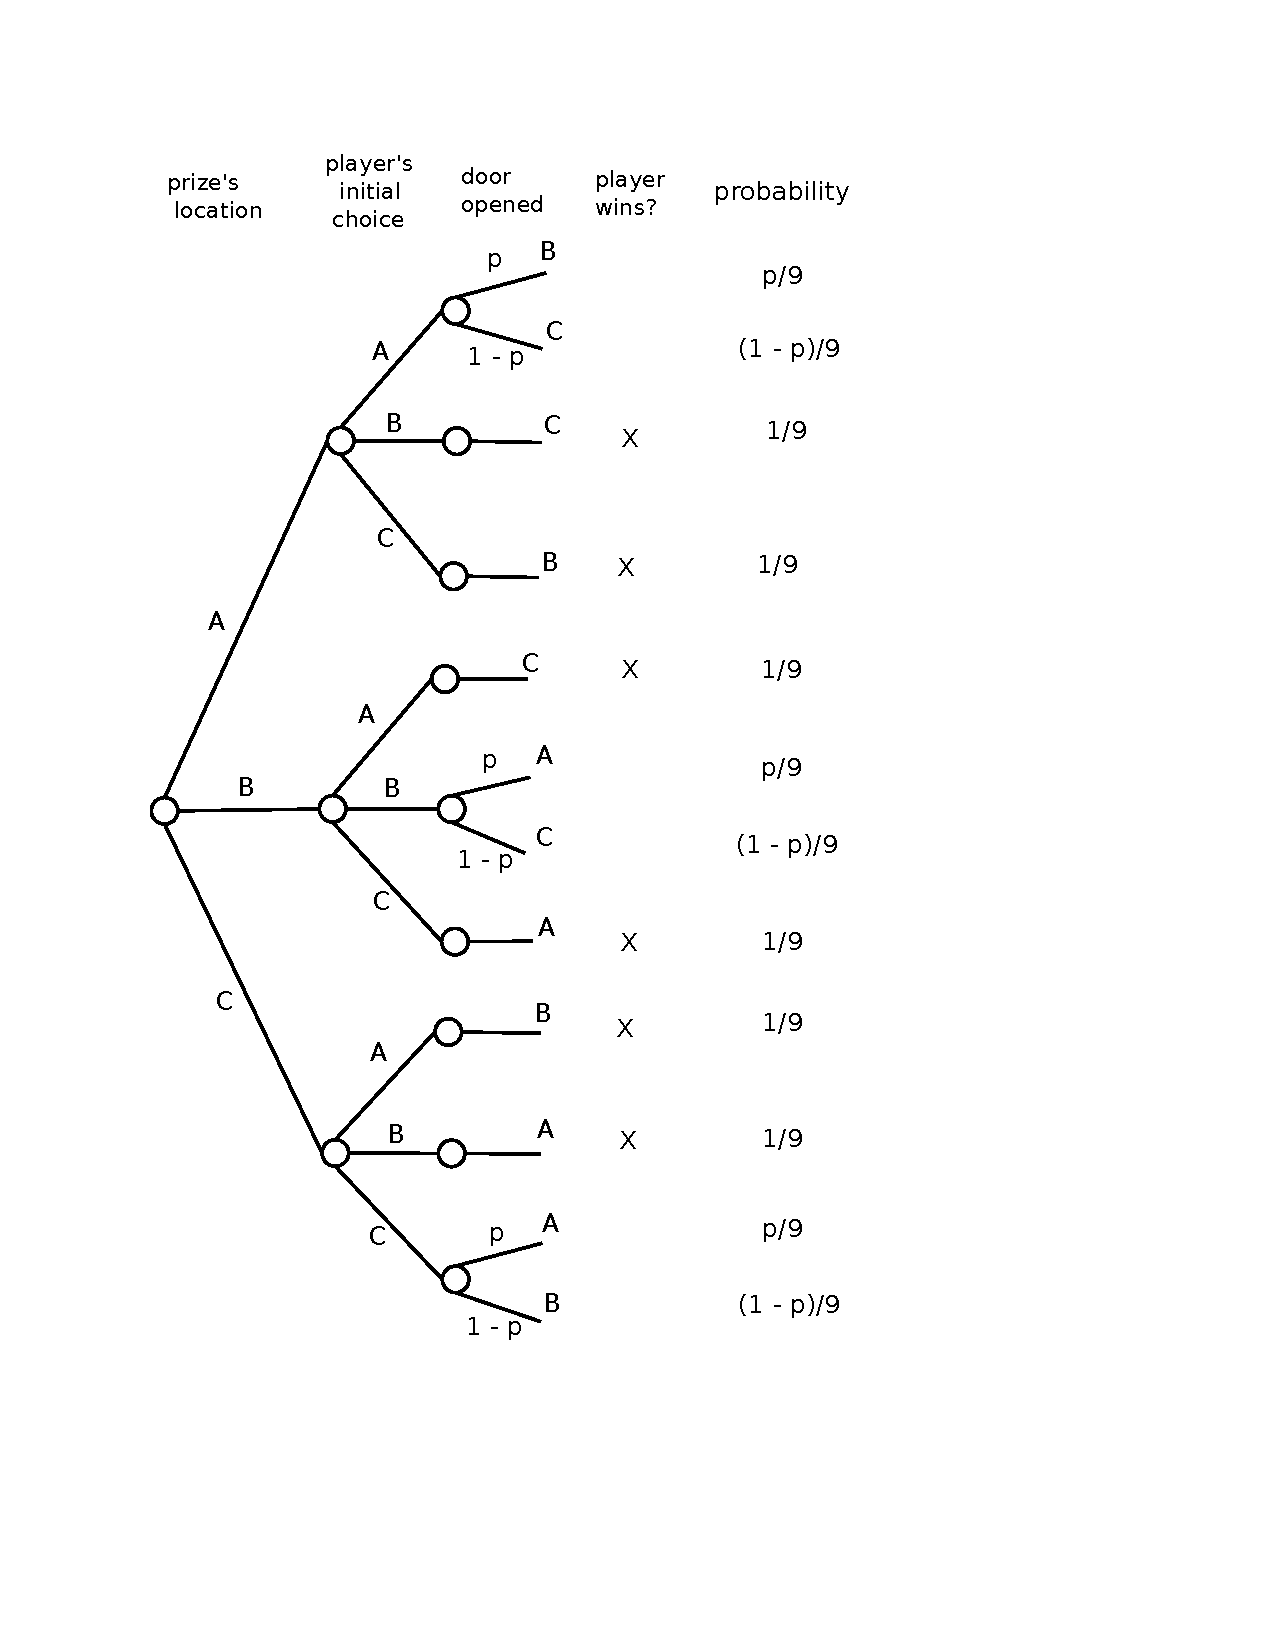
\includegraphics[scale=0.7]{carolp}
\end{center}

Therefore the probability remains $2/3$. Notice the parameter $p$ has no effect in the final formula, because if the contestant plays the ``always switch'' strategy then she will invariably lose in those situations where Carol has the option to choose among two doors.  In the solution we could even allow the parameters $p$, $q$, and $r$ rather than a single $p$, allowing Carol pick them separately, it would still make no difference. 

To analyze the original Monty Hall problem, we made the assumption ``Carol picks one of the remaining doors equally at random'', but from the two previous problems we can see this assumption was not needed in order to conclude switching wins more than half of the time. 

}

\newpage
\subsection{Optimal strategy}
So far we assumed the contestant always switches, and analyzed the outcome of the game that way. In lecture we also discussed the strategy of always sticking to the original choice. We determined that the probability of winning with the ``always stay'' is larger than the one of winning with an  ``always switch'' strategy, in fact they are complementary.

But, what if the contestant decides whether to switch or not on a case by case basis? That is, suppose the contestant makes a decision on whether to switch or to stay based on 1) Her original choice, and 2) Carol's choice of door.

 Suppose the doors are labelled A, B and C. Show ``always switching'' is optimal. (Hint: a strategy can be seen as a mapping that assigns a pair $\left(D_1, D_2 \right)$ of observations to a decision: switch to $D_3$ or stay in $D_1$. The strategy needs to be defined for all pairs $\left(A,B\right)$, $\left(A, C\right)\cdots$. You can optimize the reaction for each potential observation individually.)

\solution{
Suppose without losing generality the contestant picks door $A$ and is shown door $B$. He must decide on the basis of this information whether to switch to door $C$  or stay in $A$. Picking $A$ and observing $B$ is consistent with the prize being behind $A$ or $C$. As the tree diagram shows, we are only dealing with a subgraph of the full tree:

\begin{center}
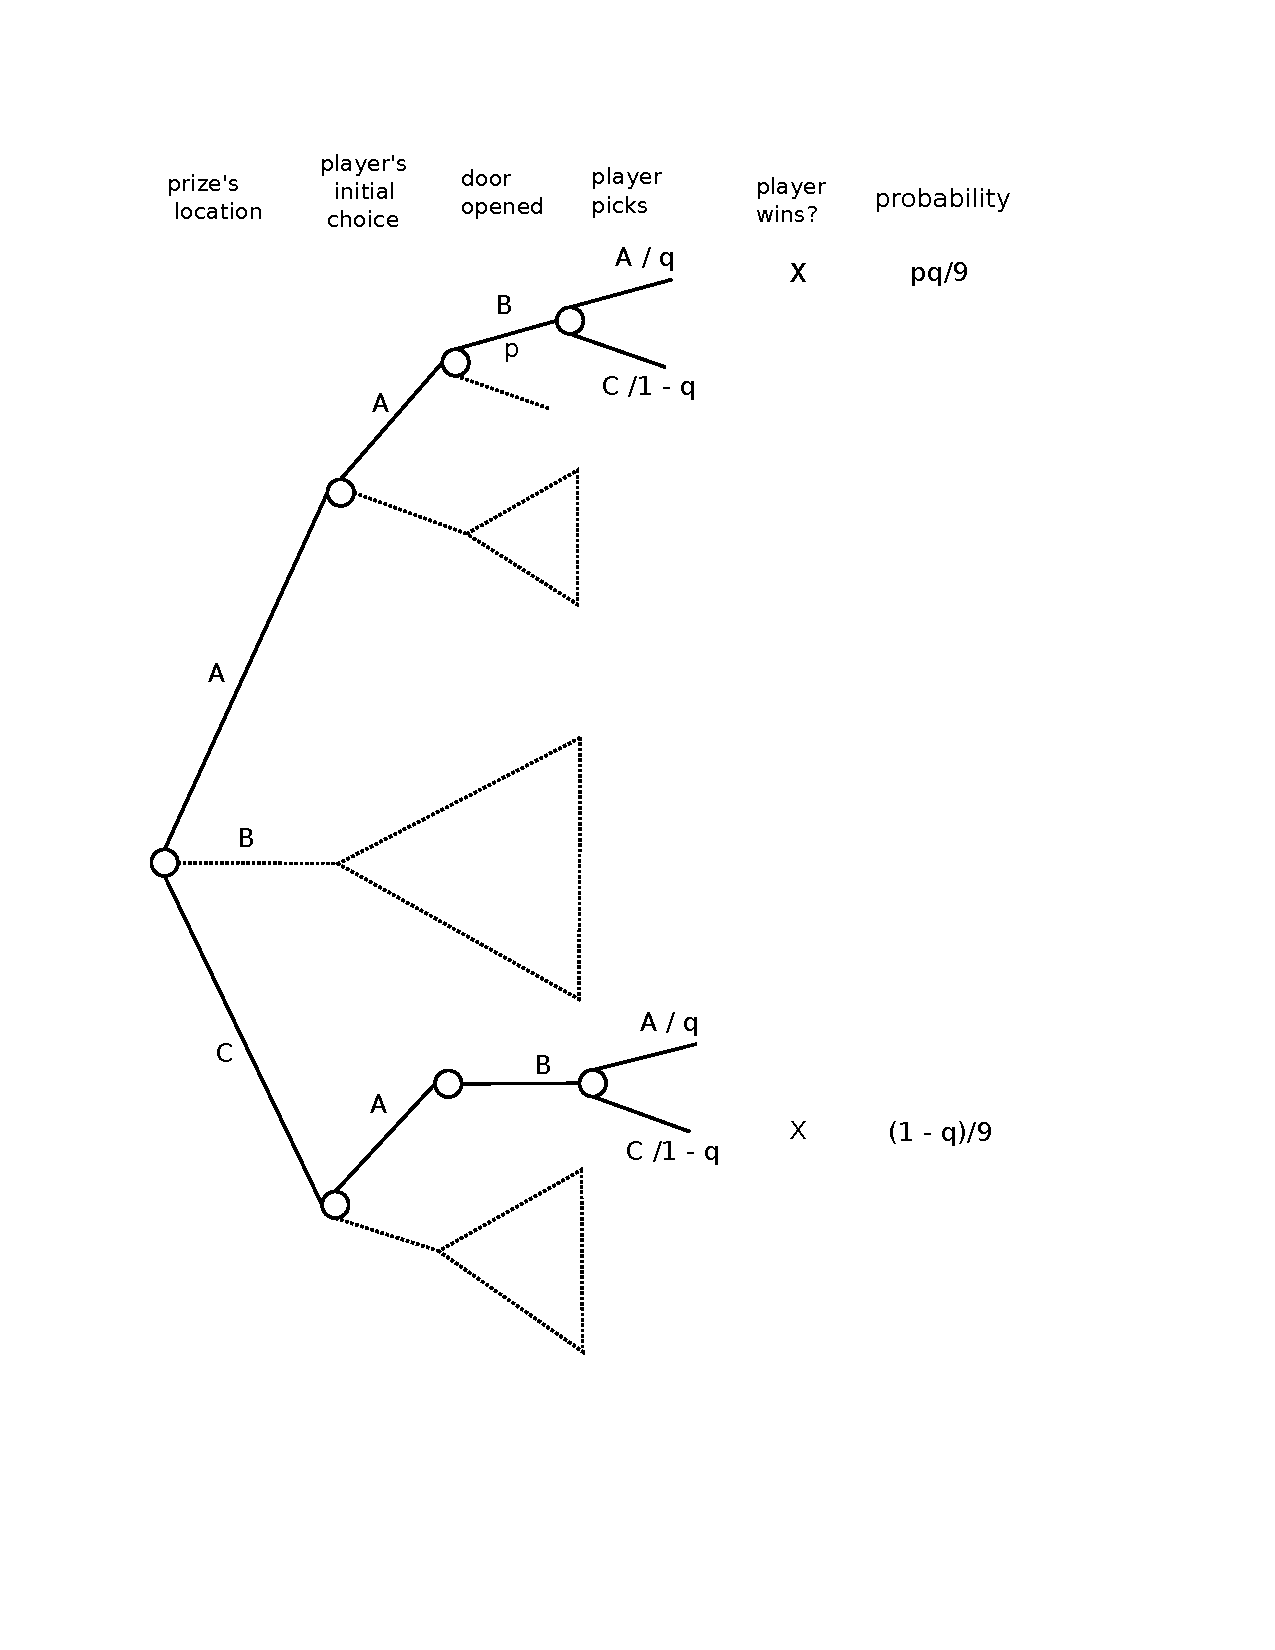
\includegraphics[scale=0.7]{subtree}
\end{center}

The diagram indicates Carol picks one door with probability $p$, and the other with probability $1-p$ when she has a choice.  The contestant has a strategy summarized of switching with probablity $q$.  When $q = 1$ we mean she will stay, when $q = 0$ we mean she will switch. 

The total probability of winning will include two contributions from the two illustrated branches, for a total of $(pq + 1-q)/9$. For a given $p$, if the contestant decides to move $q$ to $0$, the contribution becomes $1/9$. If the contestant moves $q$ towards $1$, she gets a contribution of $p/9$.  Since $p \leq 1$, then switching will at worst be as good. Notice also that any other value of $q$ in between $0$ and $1$ will not be optimal (since it is an average of the two extremes). Hence, having $q = 0$ is the best choice, no matter what $p$ is.   

In this way, the contestant can optimize her choice for every possible pair of observations. By symmetry you can see the answers will be the same: switch. Hence the overall optimal strategy is ``always switch''.  This result is actually a little stronger than what was suggested in the problem, in which you were only asked to consider the extreme values of $q = 1$ and $q = 0$.

Contrast this with the $4$ door version of the problem, where Mergatroid has a strategy that performs better than switching. 
}

\end{document}

